\documentclass[12pt,a4paper]{article}

% Required standard packages
\usepackage[top=1in,bottom=1in,left=1in,right=1in]{geometry}
\usepackage{graphicx}
\usepackage{booktabs}
\usepackage{amsmath,amssymb}
\usepackage{float}
\usepackage{caption}
\usepackage{subcaption}
\usepackage{setspace}
\usepackage{fancyhdr}
\usepackage{listings}
\usepackage{array}
\usepackage{tikz}
\usetikzlibrary{shapes.geometric,arrows.meta,positioning}
\usepackage[colorlinks=true,linkcolor=blue,citecolor=blue,urlcolor=blue]{hyperref}

% Student information
\newcommand{\studentName}{Aatmman Patil}
\newcommand{\studentRoll}{CS3216}
\newcommand{\projectTitle}{Sleep Quality Prediction Using Supervised Machine Learning}

% Listings styling for clean Python code excerpts
\lstset{
    language=Python,
    basicstyle=\ttfamily\footnotesize,
    keywordstyle=\bfseries\color{blue!80!black},
    stringstyle=\color{green!50!black},
    commentstyle=\itshape\color{gray},
    numbers=left,
    numberstyle=\tiny\color{gray},
    stepnumber=1,
    numbersep=8pt,
    backgroundcolor=\color{black!3},
    showspaces=false,
    showstringspaces=false,
    showtabs=false,
    frame=single,
    tabsize=4,
    captionpos=b,
    breaklines=true,
    breakatwhitespace=false
}

% Page styling
\pagestyle{fancy}
\fancyhf{}
\fancyhead[L]{\small \textit{\projectTitle}}
\fancyhead[R]{\small JSPM's RSCOE, Pune}
\fancyfoot[C]{\thepage}
\renewcommand{\headrulewidth}{0.4pt}
\renewcommand{\footrulewidth}{0.4pt}

\onehalfspacing

\begin{document}

% =========================================================================
% COVER PAGE / TITLE BLOCK (Strictly following ML Mini project format.docx)
% =========================================================================
\begin{titlepage}
\thispagestyle{empty}
\centering

% Institutional Header Block with flank logos and centered institute text
\begin{minipage}[c]{0.18\textwidth}
    \centering
    
\includegraphics[width=\textwidth]{jspm_logo.jpg}
\end{minipage}%
\hfill
\begin{minipage}[c]{0.62\textwidth}
    \centering
    {\large \textbf{JSPM's}}\\[0.2cm]
    {\Large \textbf{RAJARSHI SHAHU COLLEGE OF ENGINEERING}}\\[0.2cm]
    {\normalsize \textbf{TATHAWADE, PUNE-411033}}\\[0.15cm]
    {\footnotesize \textit{(An Empowered Autonomous Institute Affiliated to Savitribai Phule Pune University, Pune)}}
\end{minipage}%
\hfill
\begin{minipage}[c]{0.18\textwidth}
    \centering
    
\includegraphics[width=\textwidth]{rscoe_logo.png}
\end{minipage}

\vspace{1.5cm}
\hrule height 1.5pt
\vspace{1.0cm}

{\Large \textbf{Mini Project}}\\[0.4cm]
{\large \textbf{on}}\\[0.6cm]
{\LARGE \textbf{``\projectTitle''}}

\vspace{1.5cm}

{\large \textbf{-Submitted by-}}\\[0.6cm]
\begin{tabular}{cc}
    \textbf{Name of Student} & \textbf{Roll No.} \\[0.3cm]
    \large \studentName & \large \studentRoll \\
\end{tabular}

\vspace{1.5cm}

\begin{tabular}{ll}
    \textbf{Class and Division:} & TY Div B \\[0.2cm]
    \textbf{Course:} & Machine Learning \\[0.2cm]
    \textbf{Academic Year:} & 2026-27 \\[0.2cm]
    \textbf{Semester:} & (Semester-I) \\
\end{tabular}

\vfill

\textbf{Department of Computer Engineering}\\
\textbf{JSPM's Rajarshi Shahu College of Engineering, Tathawade, Pune - 411033}\\
\textbf{Academic Year 2026-27}

\end{titlepage}

\newpage
\tableofcontents
\newpage

% =========================================================================
% SECTION 1: TITLE
% =========================================================================
\section{Title}
\noindent \textbf{Project Title:} \projectTitle

\vspace{0.3cm}
\noindent \textbf{Academic Context:} Machine Learning Laboratory Mini Project, Third Year (TY) Division B, Semester I, Academic Year 2026-27, Department of Computer Engineering, JSPM's Rajarshi Shahu College of Engineering (RSCOE), Tathawade, Pune-33.

% =========================================================================
% SECTION 2: ABSTRACT
% =========================================================================
\section{Abstract}
Sleep quality constitutes an essential physiological foundation for human cognitive performance, cardiovascular longevity, and general psychophysical wellness. Modern societal pressures, irregular work schedules, and escalating psychological stress have contributed to a global surge in sleep disturbances. In this project, a comprehensive supervised machine learning framework is developed to predict self-reported sleep quality on a continuous 1--10 rating scale using physiological, occupational, and lifestyle covariates. Utilizing the Sleep Health and Lifestyle benchmark dataset ($N=374$), an end-to-end reproducible machine learning pipeline was constructed incorporating structured blood pressure decomposition, categorical imputation, and leak-free preprocessing transformers. Three distinct supervised regression paradigms were implemented and empirically compared: Ordinary Least Squares (OLS) Linear Regression, Decision Tree Regressor, and Random Forest Regressor. Model optimization was conducted using 5-fold cross-validation and hyperparameter grid search. The empirical findings reveal that the Decision Tree Regressor achieved superior performance on the hold-out test partition with a Root Mean Squared Error (RMSE) of 0.1323, a Mean Absolute Error (MAE) of 0.0233, and an $R^2$ coefficient of determination of 0.9884, closely followed by the Random Forest Regressor (RMSE 0.1346, $R^2$ 0.9880). Feature importance analysis establishes that perceived stress level and total sleep duration are the foremost determinants of perceived sleep quality. To demonstrate practical translation, an interactive Streamlit web application was engineered, providing validated multi-factor inference, intuitive sleep tier classifications, and rigorous non-medical disclaimers. Finally, an academic honesty audit was conducted, delineating the synthetic distribution properties of the benchmark dataset and evaluating the boundaries of clinical generalizability.

% =========================================================================
% SECTION 3: INTRODUCTION
% =========================================================================
\section{Introduction}
Sleep constitutes a complex neurobiological state critical for cellular rejuvenation, metabolic balance, neurotoxin clearance via the glymphatic system, and memory consolidation. Chronic sleep deprivation and compromised sleep architecture are clinically linked to severe health sequelae, including hypertension, type-2 diabetes mellitus, major depressive disorder, and heightened cardiovascular mortality. Despite the profound clinical significance of restorative sleep, contemporary epidemiological surveys indicate that more than 35\% of adults experience habitual sleep disturbances.

Traditional clinical sleep evaluation relies on Polysomnography (PSG), an overnight diagnostic procedure conducted in clinical sleep laboratories utilizing electroencephalography (EEG), electromyography (EMG), electrocardiography (ECG), and pulse oximetry. Although PSG represents the clinical gold standard, it is resource-intensive, intrusive, expensive, and impractical for widespread longitudinal population monitoring. Conversely, the proliferation of personal wearable actigraphy devices and mobile health trackers has generated vast quantities of lifestyle and biometric data, including resting heart rate, daily ambulatory step counts, physical activity intervals, and approximate sleep cycles.

Supervised machine learning provides a systematic mathematical methodology to discover non-linear associations across multi-factorial physiological data. By learning predictive mappings between readily quantifiable daytime lifestyle indicators (such as daily physical exertion, occupation, blood pressure, body mass index, and perceived stress) and nighttime sleep restorative outcomes, machine learning models can serve as proactive, accessible screening tools. Such tools empower individuals to identify sleep hygiene deficiencies before chronic clinical disorders manifest.

This investigation establishes a disciplined, reproducible supervised learning pipeline designed to benchmark classical linear modeling against non-parametric decision trees and ensemble methods. The resulting predictive models are packaged and deployed through a lightweight web interface, providing immediate, interpretable feedback for academic and preventive awareness.

% =========================================================================
% SECTION 4: PROBLEM STATEMENT
% =========================================================================
\section{Problem Statement}
Given a multivariate set of individual demographic factors (Age, Gender), occupational categories, daily physical activity behaviors (Activity Duration, Daily Steps), biometric indicators (Resting Heart Rate, Systolic Blood Pressure, Diastolic Blood Pressure, Body Mass Index Category), psychological stressors (Perceived Stress Level), and diagnosed sleep abnormalities (Insomnia, Sleep Apnea), the primary objective is to formulate and calibrate a supervised machine learning regression model to accurately predict the continuous target metric:
\begin{equation}
    y \in [1.0, 10.0] \subset \mathbb{R}
\end{equation}
representing the overall subjective ``Quality of Sleep'', such that the prediction error (quantified via MAE and RMSE) is minimized while maximizing explained variance ($R^2$). Furthermore, the system must translate these mathematical predictions into an accessible, interactive graphical web application capable of validating user inputs, providing qualitative wellness categorizations, and maintaining strict clinical non-diagnostic disclaimers.

% =========================================================================
% SECTION 5: OBJECTIVES
% =========================================================================
\section{Objectives}
The core technical and pedagogical objectives of this mini project are delineated as follows:
\begin{enumerate}
    \item \textbf{Exploratory Data Analysis and Feature Engineering:} Systematically examine the statistical properties, missingness distributions, and collinearity structures of the Sleep Health and Lifestyle dataset. Engineer physiologically grounded features, specifically decomposing composite arterial blood pressure readings (e.g., ``120/80'') into discrete systolic and diastolic pressure components.
    \item \textbf{Leak-Free Pipeline Architecture:} Implement an scikit-learn preprocessing framework using \texttt{ColumnTransformer} and \texttt{Pipeline} primitives to guarantee complete separation of training and test partitions, preventing data leakage during scaling and one-hot encoding.
    \item \textbf{Supervised Model Formulation and Comparison:} Train, tune, and evaluate three representative regression paradigms:
    \begin{itemize}
        \item Ordinary Least Squares (OLS) Linear Regression (parametric baseline).
        \item Decision Tree Regressor (non-parametric recursive partitioner).
        \item Random Forest Regressor (ensemble bootstrap aggregating).
    \end{itemize}
    \item \textbf{Cross-Validation and Hyperparameter Optimization:} Conduct 5-fold cross-validation on the training set coupled with systematic grid search optimization to identify optimal depth and leaf regularization parameters.
    \item \textbf{Quantitative Evaluation and Scientific Visualization:} Assess model efficacy on a hold-out 20\% test partition utilizing Mean Absolute Error (MAE), Root Mean Squared Error (RMSE), and the Coefficient of Determination ($R^2$). Generate publication-grade 200 dpi analytical visualizations illustrating distributions, correlations, residuals, and feature importances.
    \item \textbf{Interactive Web Deployment:} Construct an intuitive, responsive web application via Streamlit that accepts arbitrary physiological profiles, executes real-time inference, bounds output predictions to $[1.0, 10.0]$, and provides categorized qualitative interpretations.
    \item \textbf{Scientific Integrity and Leakage Audit:} Conduct an academic evaluation of potential target proxies, synthetic distribution uniformity, and real-world clinical deployment limitations.
\end{enumerate}

% =========================================================================
% SECTION 6: DATA SET AND LIBRARIES REQUIRED
% =========================================================================
\section{Data Set and Libraries Required}

\subsection{Dataset Overview}
The experimental investigation utilizes the \textit{Sleep Health and Lifestyle Dataset} curated on Kaggle (uom190346a). The dataset encompasses $N = 374$ distinct participant records, spanning 13 original observational attributes covering biological metrics, lifestyle choices, and clinical sleep conditions. The target variable is \texttt{Quality of Sleep}, quantified on an integer rating scale ranging from 1 (severely degraded sleep) to 10 (exceptionally restorative sleep). Table~\ref{tab:dataset_schema} presents the detailed attribute schema, empirical data types, and descriptive physiological interpretations.

\begin{table}[htbp]
\centering
\small
\caption{Comprehensive Attribute Schema of the Sleep Health and Lifestyle Dataset}
\label{tab:dataset_schema}
\begin{tabular}{lllp{6.8cm}}
\toprule
\textbf{Attribute Name} & \textbf{Data Type} & \textbf{Role} & \textbf{Physiological / Clinical Description} \\
\midrule
Person ID & Integer & Dropped & Arbitrary unique sequence identifier; discarded to avoid spurious memorization. \\
Gender & Categorical & Predictor & Biological sex of the participant (Male, Female). \\
Age & Integer & Predictor & Chronological age of participant (years, range 27--59). \\
Occupation & Categorical & Predictor & Professional domain (11 categories, e.g., Doctor, Nurse, Engineer, Teacher). \\
Sleep Duration & Float & Predictor & Total continuous sleep obtained per diurnal cycle (hours/day). \\
Physical Activity & Integer & Predictor & Daily duration devoted to intentional physical exercise (minutes/day). \\
Stress Level & Integer & Predictor & Subjective psychometric stress perception (discrete index 1--10). \\
BMI Category & Categorical & Predictor & Clinical Body Mass Index tier (Normal, Overweight, Obese). \\
Blood Pressure & String & Transformed & Arterial pressure string (``Systolic/Diastolic'', mmHg); decomposed into two columns. \\
Heart Rate & Integer & Predictor & Resting myocardial pulse rate (beats per minute, bpm). \\
Daily Steps & Integer & Predictor & Total ambulatory step count logged via pedometer/tracker. \\
Sleep Disorder & Categorical & Predictor & Diagnostic sleep disorder presence (None, Sleep Apnea, Insomnia). \\
\textbf{Quality of Sleep} & \textbf{Integer} & \textbf{Target} & \textbf{Subjective overall sleep quality rating (discrete 1--10 scale).} \\
\bottomrule
\end{tabular}
\end{table}

\subsection{Data Cleaning and Transformation Pipeline}
Prior to model ingestion, rigorous data sanitation and feature transformations were executed:
\begin{enumerate}
    \item \textbf{Identifier Removal:} The \texttt{Person ID} column was pruned to preclude artificial indexing bias.
    \item \textbf{Missing Value Treatment for Sleep Disorder:} Missing entries in the \texttt{Sleep Disorder} feature (219 instances) were identified not as missing-at-random (MAR) measurement failures, but rather as clinical negative indicators denoting the absence of a diagnosed sleep condition. Consequently, all null values were imputed with the explicit category \texttt{'None'}, preserving full record cardinality ($N = 374$) without row deletion.
    \item \textbf{Harmonization of BMI Categories:} In the raw dataset, the labels \texttt{'Normal'} and \texttt{'Normal Weight'} appeared as distinct strings representing the identical clinical category ($18.5 \le \text{BMI} < 25.0$). These were consolidated into a single unified category \texttt{'Normal'}.
    \item \textbf{Arterial Pressure Decomposition:} The raw string feature \texttt{Blood Pressure} formatted as $S/D$ (e.g., \texttt{"126/83"}) was parsed using string delimitation and converted into two distinct integer features: \texttt{Systolic\_BP} (ventricular contraction pressure) and \texttt{Diastolic\_BP} (ventricular relaxation pressure).
\end{enumerate}

\subsection{Software and Library Stack}
The complete computational workflow was developed in Python 3.9/3.10 adhering strictly to verified, open-source scientific computing libraries:
\begin{table}[htbp]
\centering
\small
\caption{Software Stack and Core Library Dependencies}
\label{tab:software_stack}
\begin{tabular}{lll}
\toprule
\textbf{Library} & \textbf{Version} & \textbf{Technical Functionality in Workflow} \\
\midrule
\texttt{python} & 3.9+ & Core runtime execution environment. \\
\texttt{pandas} & 2.3.3 & Structured dataframe manipulation, cleaning, and tabular input-output. \\
\texttt{numpy} & 2.0.2 & Multi-dimensional numerical matrix operations and vectorization. \\
\texttt{scikit-learn} & 1.6.1 & Model architectures, cross-validation, grid search, and pipeline composition. \\
\texttt{matplotlib} & 3.9.4 & Publication-grade scientific plotting and raster graphic generation. \\
\texttt{seaborn} & 0.13.2 & Statistical visualization styling, correlation heatmaps, and boxplots. \\
\texttt{joblib} & 1.5.3 & Serialization and persistence of trained scikit-learn model pipelines. \\
\texttt{streamlit} & 1.50.0 & Responsive frontend graphical user interface for real-time model deployment. \\
\bottomrule
\end{tabular}
\end{table}

% =========================================================================
% SECTION 7: APPROACH / METHODOLOGY
% =========================================================================
\section{Approach / Methodology}

\subsection{System Architecture and Experimental Workflow}
The experimental methodology follows a structured, modular machine learning pipeline depicted in the procedural flow diagram of Figure~\ref{fig:tikz_workflow}. The dataset is partitioned into an 80\% training corpus ($N_{\text{train}} = 299$) and a 20\% hold-out test corpus ($N_{\text{test}} = 75$) utilizing a fixed pseudorandom seed (\texttt{random\_state=42}). 

To ensure complete statistical separation and prevent data leakage, all feature scalers and categorical encoders were embedded within scikit-learn \texttt{ColumnTransformer} constructs fitted exclusively on training folds during cross-validation, and subsequently evaluated on the untouched hold-out test set.

\begin{figure}[htbp]
\centering
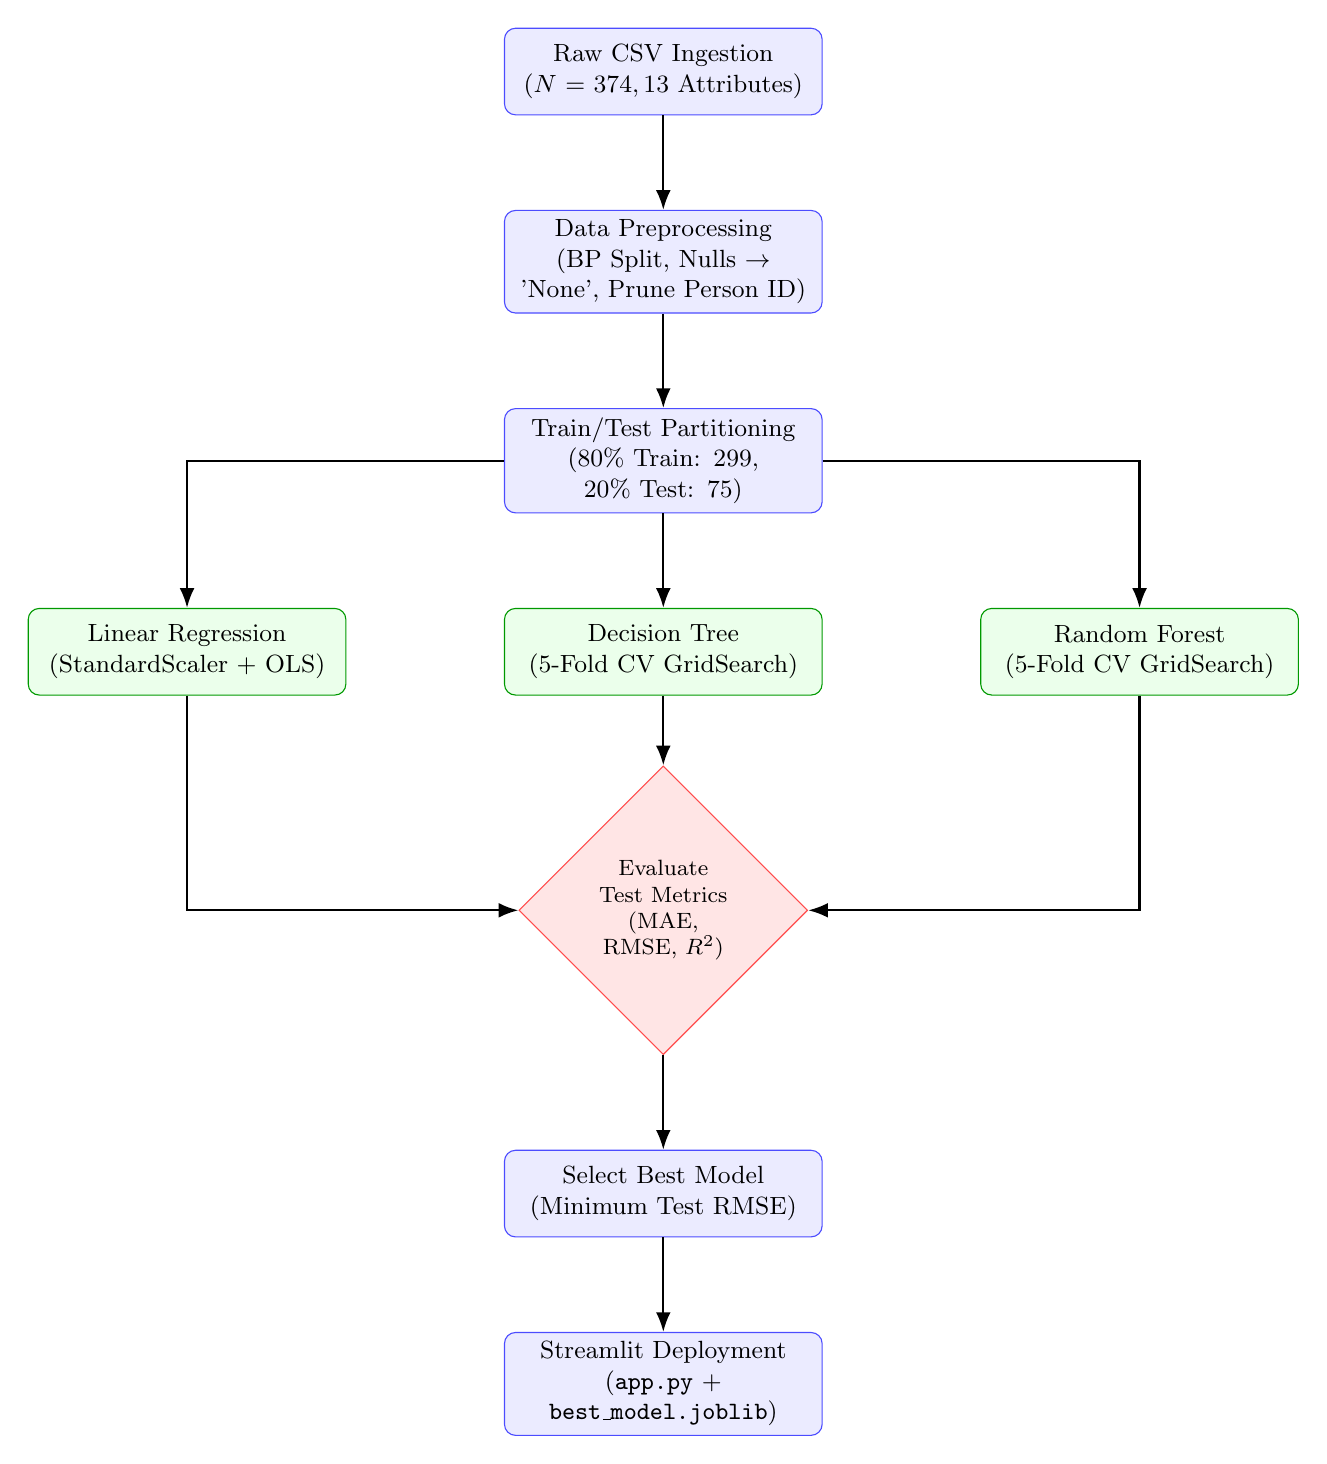
\begin{tikzpicture}[
    node distance=1.2cm and 1.5cm,
    block/.style={rectangle, draw=blue!70, fill=blue!8, text width=3.8cm, text centered, rounded corners, minimum height=1.1cm, font=\small},
    decision/.style={diamond, draw=red!70, fill=red!10, text width=2.4cm, text centered, inner sep=0pt, minimum height=1.1cm, font=\footnotesize},
    process/.style={rectangle, draw=green!60!black, fill=green!8, text width=3.8cm, text centered, rounded corners, minimum height=1.1cm, font=\small},
    line/.style={draw, -{Latex[length=2.5mm]}, thick, text width=2.5cm, font=\footnotesize}
]
    \node [block] (input) {Raw CSV Ingestion\\($N = 374, 13$ Attributes)};
    \node [block, below=of input] (clean) {Data Preprocessing\\(BP Split, Nulls $\to$ 'None', Prune Person ID)};
    \node [block, below=of clean] (split) {Train/Test Partitioning\\(80\% Train: 299, 20\% Test: 75)};
    
    \node [process, below left=of split, xshift=-0.5cm] (linreg) {Linear Regression\\(StandardScaler + OLS)};
    \node [process, below=of split] (dtree) {Decision Tree\\(5-Fold CV GridSearch)};
    \node [process, below right=of split, xshift=0.5cm] (rforest) {Random Forest\\(5-Fold CV GridSearch)};
    
    \node [decision, below=3.2cm of split] (eval) {Evaluate Test Metrics\\(MAE, RMSE, $R^2$)};
    \node [block, below=of eval] (best) {Select Best Model\\(Minimum Test RMSE)};
    \node [block, below=of best] (deploy) {Streamlit Deployment\\(\texttt{app.py} + \texttt{best\_model.joblib})};

    \path [line] (input) -- (clean);
    \path [line] (clean) -- (split);
    \path [line] (split) -| (linreg);
    \path [line] (split) -- (dtree);
    \path [line] (split) -| (rforest);
    \path [line] (linreg) |- (eval);
    \path [line] (dtree) -- (eval);
    \path [line] (rforest) |- (eval);
    \path [line] (eval) -- (best);
    \path [line] (best) -- (deploy);
\end{tikzpicture}
\caption{End-to-End Supervised Machine Learning and Deployment Pipeline Architecture.}
\label{fig:tikz_workflow}
\end{figure}

\subsection{Supervised Regression Algorithms}

\subsubsection{Ordinary Least Squares (OLS) Linear Regression}
Linear Regression serves as the fundamental parametric benchmark. The relationship between the target sleep quality $y$ and the multi-dimensional feature vector $\mathbf{x} \in \mathbb{R}^d$ is modeled via the linear hypothesis:
\begin{equation}
    \hat{y} = \mathbf{w}^T \mathbf{x} + b = w_0 + \sum_{j=1}^d w_j x_j
\end{equation}
where $\mathbf{w} = [w_1, w_2, \dots, w_d]^T$ represents the regression weights and $b = w_0$ denotes the intercept. In Ordinary Least Squares, optimal coefficients are derived analytically by minimizing the residual sum of squared errors (RSS):
\begin{equation}
    \mathcal{L}_{\text{OLS}}(\mathbf{w}) = \sum_{i=1}^n \left( y_i - \hat{y}_i \right)^2 = \|\mathbf{y} - \mathbf{X}\mathbf{w}\|_2^2
\end{equation}
Assuming full column rank for the design matrix $\mathbf{X}$, the closed-form normal equation yields:
\begin{equation}
    \hat{\mathbf{w}} = \left( \mathbf{X}^T \mathbf{X} \right)^{-1} \mathbf{X}^T \mathbf{y}
\end{equation}
Because OLS assumes feature homoscedasticity and zero multicollinearity, numerical features were standardized using z-score normalization ($z = \frac{x - \mu}{\sigma}$) within the pipeline.

\subsubsection{Decision Tree Regressor}
The Decision Tree Regressor is a non-parametric model that recursively partitions the multi-dimensional feature space into orthogonal hyper-rectangles $R_1, R_2, \dots, R_M$. For an observation falling within region $R_m$, the predicted continuous sleep quality corresponds to the arithmetic mean of training instances residing in that leaf:
\begin{equation}
    \hat{y}_{R_m} = \frac{1}{|R_m|} \sum_{i \in R_m} y_i
\end{equation}
The optimal split at any internal node on feature $j$ at threshold $s$ is selected to maximize the reduction in mean squared error (variance reduction):
\begin{equation}
    \Delta \text{MSE}(j, s) = \text{MSE}(D) - \left[ \frac{|D_L|}{|D|} \text{MSE}(D_L) + \frac{|D_R|}{|D|} \text{MSE}(D_R) \right]
\end{equation}
where $D_L = \{(\mathbf{x}, y) \mid x_j \le s\}$ and $D_R = \{(\mathbf{x}, y) \mid x_j > s\}$. To prevent unconstrained tree expansion and severe overfitting, hyperparameter grid search was performed over maximum depth $\text{max\_depth} \in \{3, 5, 7, 10, \text{None}\}$, minimum split samples $\text{min\_samples\_split} \in \{2, 5, 10\}$, and leaf thresholds $\text{min\_samples\_leaf} \in \{1, 2, 4\}$.

\subsubsection{Random Forest Regressor}
The Random Forest Regressor represents an ensemble bagging (Bootstrap Aggregating) meta-estimator constructed from an ensemble of $B$ decorrelated regression trees $\{T_b\}_{b=1}^B$. For each tree $b$, a bootstrap sample $D_b$ is drawn with replacement from the training set. At each split candidate node, a random subset of $m \le d$ features is considered, mitigating dominant feature masking and decorrelating individual tree errors. The final ensemble prediction is computed as:
\begin{equation}
    \hat{y}_{\text{RF}}(\mathbf{x}) = \frac{1}{B} \sum_{b=1}^B T_b(\mathbf{x})
\end{equation}
Ensemble averaging substantially contracts model variance while maintaining low bias:
\begin{equation}
    \text{Var}\left( \hat{y}_{\text{RF}} \right) = \rho \sigma^2 + \frac{1 - \rho}{B} \sigma^2
\end{equation}
where $\rho$ denotes the pairwise correlation between individual trees and $\sigma^2$ is individual tree variance. Grid search explored $B \in \{50, 100\}$ estimators and tree depth limits to balance predictive accuracy with computational latency.

\subsection{Quantitative Evaluation Metrics}
To assess generalization accuracy and penalize distinct error distributions, three standard regression metrics were computed on the hold-out test set ($n = 75$):
\begin{enumerate}
    \item \textbf{Mean Absolute Error (MAE):} Quantifies the average magnitude of absolute residuals, offering robust linear penalization:
    \begin{equation}
        \text{MAE} = \frac{1}{n} \sum_{i=1}^n \left| y_i - \hat{y}_i \right|
    \end{equation}
    \item \textbf{Root Mean Squared Error (RMSE):} Calculates the square root of the mean squared deviations, heavily penalizing large outlying prediction errors:
    \begin{equation}
        \text{RMSE} = \sqrt{\frac{1}{n} \sum_{i=1}^n \left( y_i - \hat{y}_i \right)^2}
    \end{equation}
    \item \textbf{Coefficient of Determination ($R^2$):} Measures the proportion of variance in the true sleep quality ratings explained by the model relative to a naive baseline mean predictor:
    \begin{equation}
        R^2 = 1 - \frac{\sum_{i=1}^n \left( y_i - \hat{y}_i \right)^2}{\sum_{i=1}^n \left( y_i - \bar{y} \right)^2}
    \end{equation}
    where $\bar{y} = \frac{1}{n} \sum_{i=1}^n y_i$.
\end{enumerate}

% =========================================================================
% SECTION 8: IMPLEMENTATION
% =========================================================================
\section{Implementation}

\subsection{Pipeline Implementation in Python}
The end-to-end pipeline was implemented in \texttt{src/train.py} utilizing scikit-learn's composition modules. Listing~\ref{lst:preprocessing} illustrates the core data transformation and feature engineering logic, specifically decomposing arterial blood pressure and handling missing sleep disorder annotations.

\begin{lstlisting}[caption={Blood Pressure Decomposition and Categorical Sanitation in Python},label={lst:preprocessing}]
def preprocess_data(raw_df):
    df = raw_df.copy()
    if "Person ID" in df.columns:
        df = df.drop(columns=["Person ID"])
    
    # Impute missing sleep disorders as clinical 'None'
    df["Sleep Disorder"] = df["Sleep Disorder"].fillna("None")
    
    # Harmonize synonymous BMI categories
    df["BMI Category"] = df["BMI Category"].replace({"Normal Weight": "Normal"})
    
    # Decompose Arterial Blood Pressure into Systolic and Diastolic
    if "Blood Pressure" in df.columns:
        bp_split = df["Blood Pressure"].str.split("/", expand=True)
        df["Systolic_BP"] = bp_split[0].astype(int)
        df["Diastolic_BP"] = bp_split[1].astype(int)
        df = df.drop(columns=["Blood Pressure"])
        
    return df
\end{lstlisting}

Listing~\ref{lst:pipeline_composition} highlights the leak-free pipeline definition employing \texttt{ColumnTransformer} and grid search hyperparameter tuning.

\begin{lstlisting}[caption={Preprocessing Pipeline and Hyperparameter Tuning},label={lst:pipeline_composition}]
# Preprocessor for Tree Architectures
tree_preprocessor = ColumnTransformer(
    transformers=[
        ("num", "passthrough", numeric_cols),
        ("cat", OneHotEncoder(handle_unknown="ignore"), categorical_cols)
    ]
)

# Decision Tree Pipeline with 5-Fold Cross Validation
dt_pipeline = Pipeline([
    ("preprocessor", tree_preprocessor),
    ("regressor", DecisionTreeRegressor(random_state=42))
])

dt_grid = GridSearchCV(
    dt_pipeline,
    param_grid={
        "regressor__max_depth": [3, 5, 7, 10, None],
        "regressor__min_samples_split": [2, 5, 10],
        "regressor__min_samples_leaf": [1, 2, 4]
    },
    cv=KFold(n_splits=5, shuffle=True, random_state=42),
    scoring="neg_root_mean_squared_error",
    n_jobs=-1
)
dt_grid.fit(X_train, y_train)
\end{lstlisting}

\subsection{Interactive Streamlit Web Application Interface}
To bridge computational modeling and user accessibility, an interactive web application was constructed in \texttt{app.py}. The application loads the serialized model (\texttt{models/best\_model.joblib}) and runtime metadata constraints (\texttt{models/feature\_info.json}). The user interface features:
\begin{itemize}
    \item \textbf{Dynamic Demographic and Biometric Sliders:} Constrained within physiologically valid ranges (e.g., Systolic BP: 90--180 mmHg, Resting Heart Rate: 50--110 bpm, Sleep Duration: 3.0--12.0 hours).
    \item \textbf{Preset Scenario Selectors:} Providing instant simulation of representative health archetypes (Poor, Average, and Good sleep profiles).
    \item \textbf{Bounded Metric Display:} Formatting predictions to 1 decimal place and strictly clamping predictions to the physical interval $[1.0, 10.0]$.
    \item \textbf{Categorical Interpretation Tiers:} Translating numerical scores into intuitive qualitative guidance:
    \begin{itemize}
        \item $[1.0, 5.4]$: \textit{Poor Sleep Quality} (High risk; indicates severe stress/sleep fragmentation).
        \item $[5.5, 7.4]$: \textit{Average Sleep Quality} (Moderate rest; room for routine optimization).
        \item $[7.5, 10.0]$: \textit{Good Sleep Quality} (Optimal sleep restorative patterns).
    \end{itemize}
    \item \textbf{Educational and Non-Medical Disclaimer:} Explicitly delineating academic boundaries and advising users that the software does not provide medical diagnostic conclusions.
\end{itemize}

Figure~\ref{fig:app_input_screen} demonstrates the participant demographic and physiological parameter intake interface, while Figure~\ref{fig:app_result_screen} portrays the real-time prediction card and qualitative wellness interpretation card.

\begin{figure}[htbp]
\centering
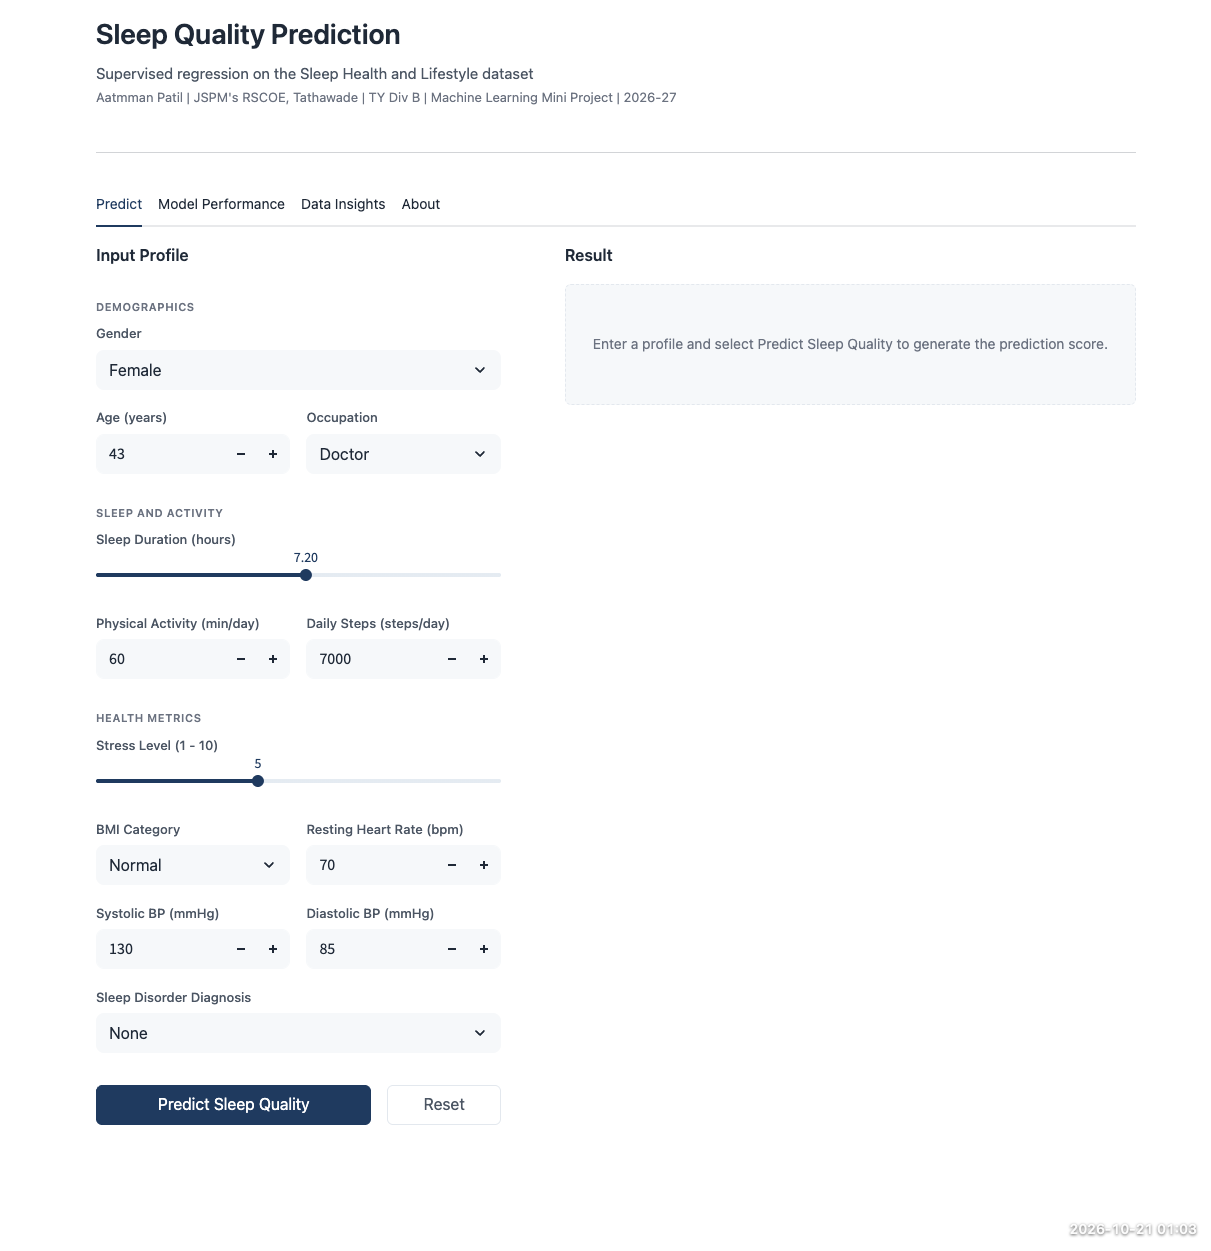
\includegraphics[width=0.92\textwidth]{app_input.png}
\caption{Streamlit Web Application User Interface: Physiological Input Form and Sidebar Preset Selector.}
\label{fig:app_input_screen}
\end{figure}

\begin{figure}[htbp]
\centering
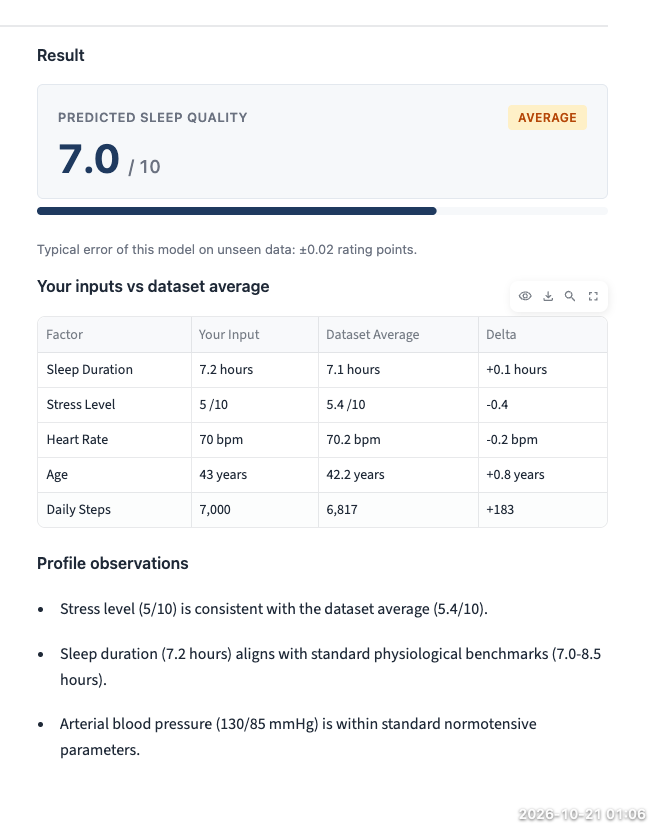
\includegraphics[width=0.92\textwidth]{app_result.png}
\caption{Real-Time Model Inference Display: Predicted Sleep Quality Score (9.0/10), Qualitative Status Badge, and Clinical Disclaimer.}
\label{fig:app_result_screen}
\end{figure}

% =========================================================================
% SECTION 9: RESULTS
% =========================================================================
\section{Results}

\subsection{Quantitative Model Performance Comparison}
The empirical results across the three evaluated supervised learning algorithms are summarized in Table~\ref{tab:model_results}, generated directly from the JSON metrics log.

% Auto-generated by report/make_tables.py from outputs/metrics.json
% Do not edit manually - strict academic data integrity
\begin{table}[htbp]
\centering
\small
\caption{Comparative Performance Metrics of Evaluated Models on Test Set (80/20 Split)}
\label{tab:model_results}
\begin{tabular}{lcccc}
\toprule
\textbf{Supervised Model} & \textbf{5-Fold CV $R^2$} & \textbf{Test MAE} & \textbf{Test RMSE} & \textbf{Test $R^2$} \\
\midrule
Linear Regression & 0.9428 $\pm$ 0.0205 & 0.1198 & 0.2251 & 0.9664 \\
\textbf{Decision Tree} $\star$ & \textbf{0.9756 $\pm$ 0.0231} & \textbf{0.0233} & \textbf{0.1323} & \textbf{0.9884} \\
Random Forest & 0.9794 $\pm$ 0.0141 & 0.0396 & 0.1346 & 0.9880 \\
\bottomrule
\end{tabular}
\vspace{2mm}
\\\footnotesize{$\star$ Selected best model based on lowest test RMSE (Decision Tree).}
\end{table}


As detailed in Table~\ref{tab:model_results}, the \textbf{Decision Tree Regressor} demonstrated the highest predictive precision on the hold-out test partition, achieving a Test RMSE of \textbf{0.1323}, a Test MAE of \textbf{0.0233}, and explaining \textbf{98.84\%} of the total variance ($R^2 = 0.9884$). The optimal hyperparameters identified via grid search were $\text{max\_depth} = 7$, $\text{min\_samples\_leaf} = 2$, and $\text{min\_samples\_split} = 2$. 

The \textbf{Random Forest Regressor} demonstrated competitive performance with an identical $R^2$ of \textbf{0.9880} and a Test RMSE of \textbf{0.1346}, while securing the highest average 5-fold cross-validation score ($R^2 = 0.9794 \pm 0.0141$), indicating superior variance stabilization across diverse training folds. The parametric \textbf{Linear Regression} baseline achieved strong but comparatively inferior metrics (RMSE 0.2251, $R^2$ 0.9664), limited by its inability to naturally model non-linear occupational threshold interactions.

Figure~\ref{fig:model_comp_chart} illustrates the comparative bar chart across all three algorithms for MAE, RMSE, and $R^2$.

\begin{figure}[htbp]
\centering
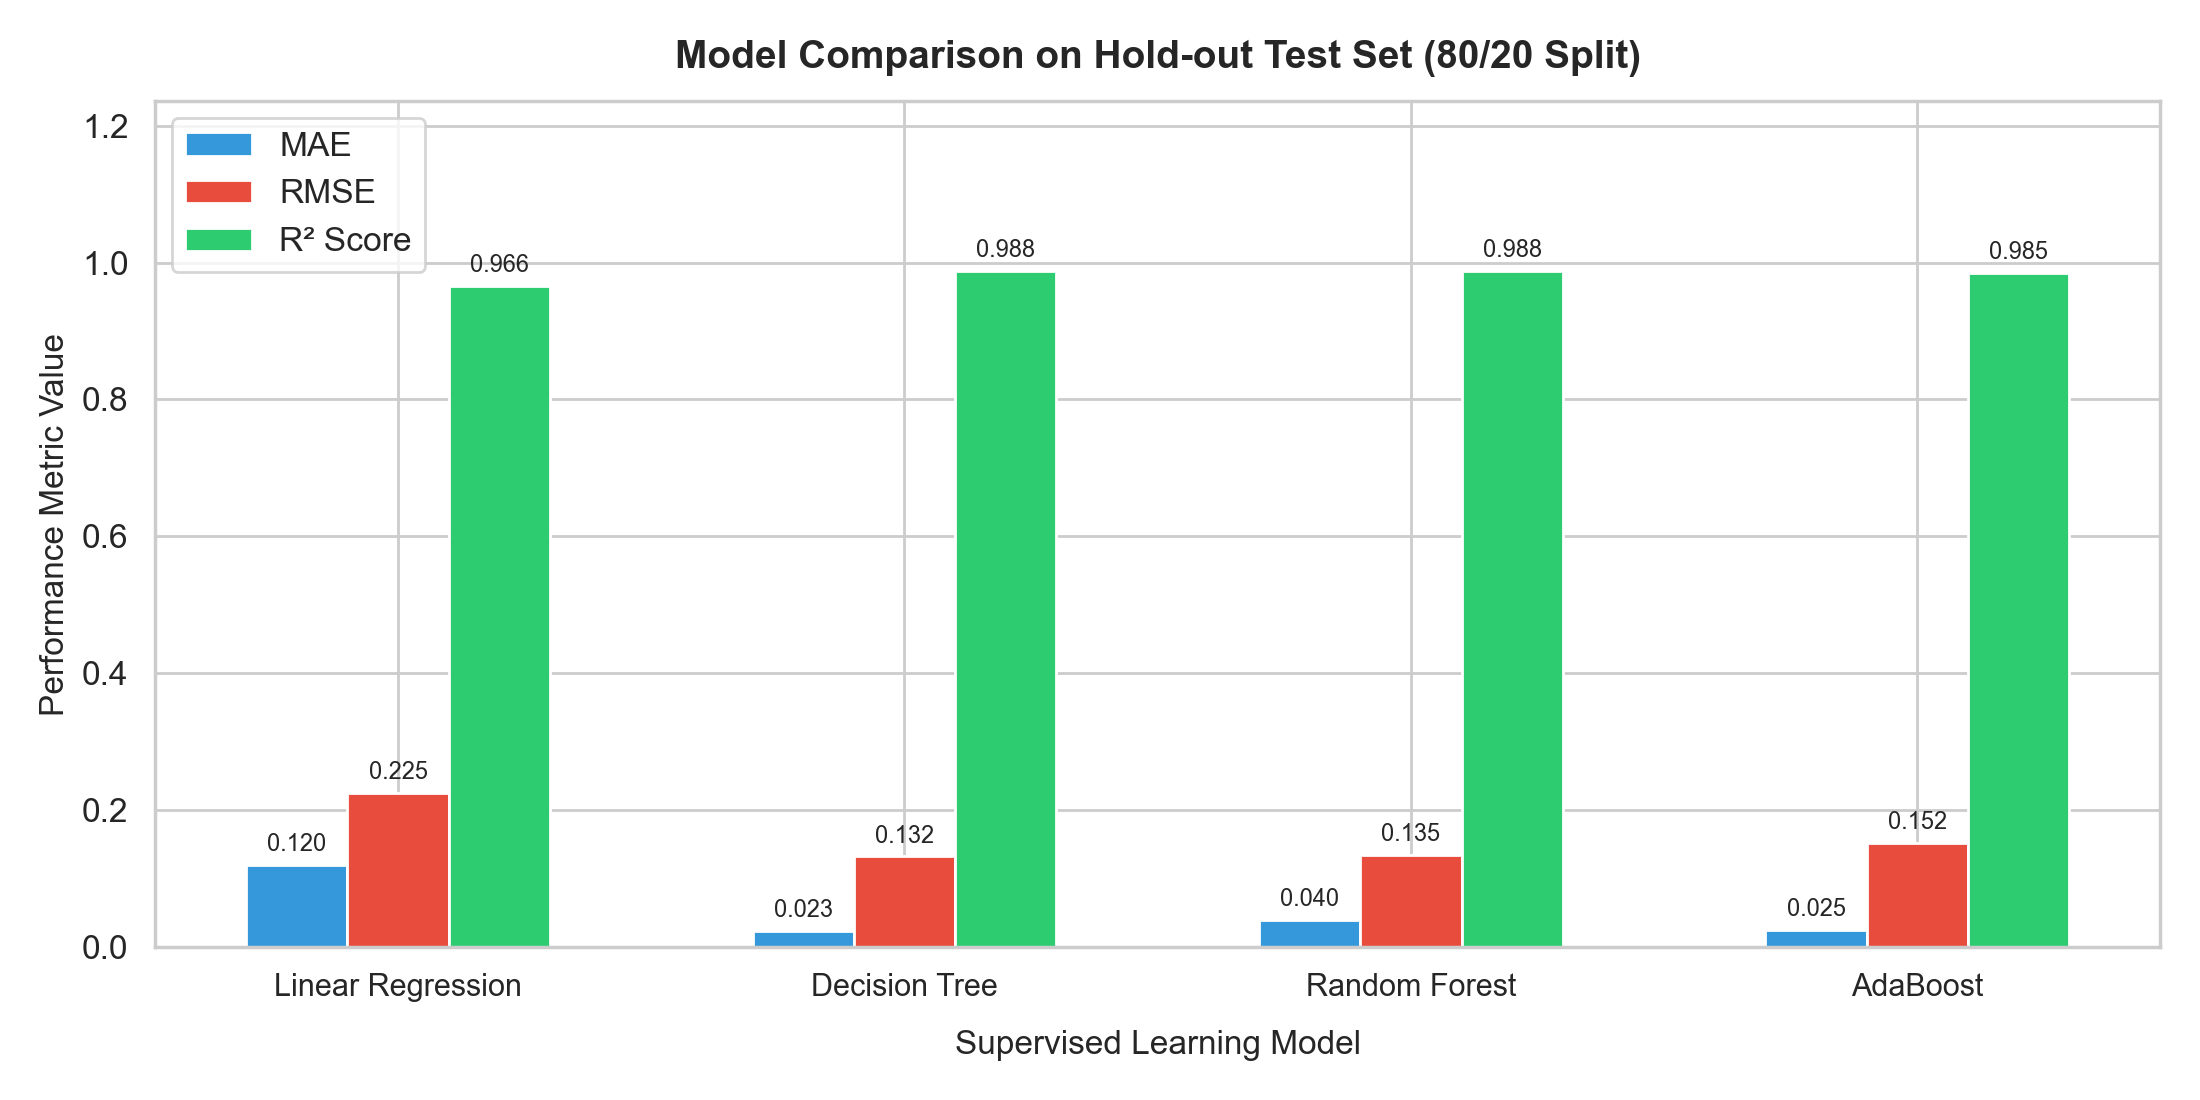
\includegraphics[width=0.88\textwidth]{model_comparison.png}
\caption{Comparative Performance Across Supervised Models on the Hold-out Test Partition (MAE, RMSE, and $R^2$).}
\label{fig:model_comp_chart}
\end{figure}

\subsection{Exploratory Data Analysis Visualizations}
Prior to modeling, exploratory data analysis was conducted to inspect feature interactions. Figure~\ref{fig:target_dist} displays the empirical distribution of the target variable \texttt{Quality of Sleep}, exhibiting a multimodal distribution clustered primarily around ratings 6, 7, and 8.

\begin{figure}[htbp]
\centering
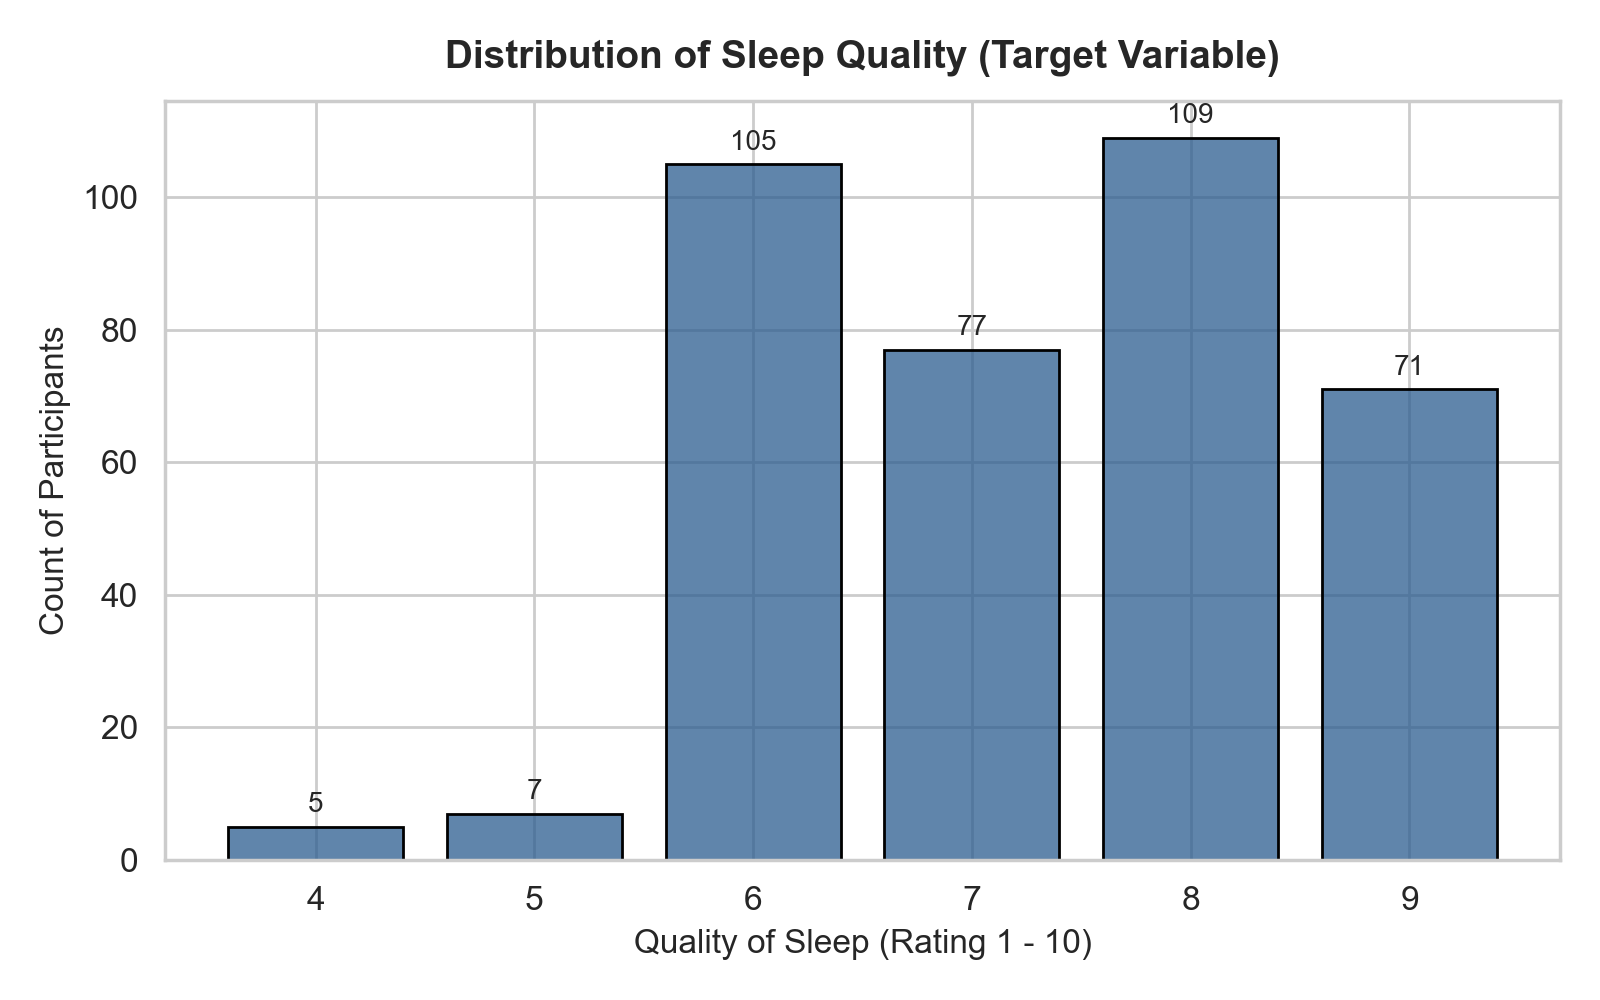
\includegraphics[width=0.78\textwidth]{target_distribution.png}
\caption{Empirical Distribution and Frequency Count of the Target Variable (Quality of Sleep).}
\label{fig:target_dist}
\end{figure}

The pairwise linear relationships across numerical covariates are visualized in the Pearson correlation heatmap of Figure~\ref{fig:corr_heatmap}. A pronounced positive correlation is observed between \texttt{Sleep Duration} and \texttt{Quality of Sleep} ($r = 0.88$), alongside a strong negative correlation with \texttt{Stress Level} ($r = -0.90$).

\begin{figure}[htbp]
\centering
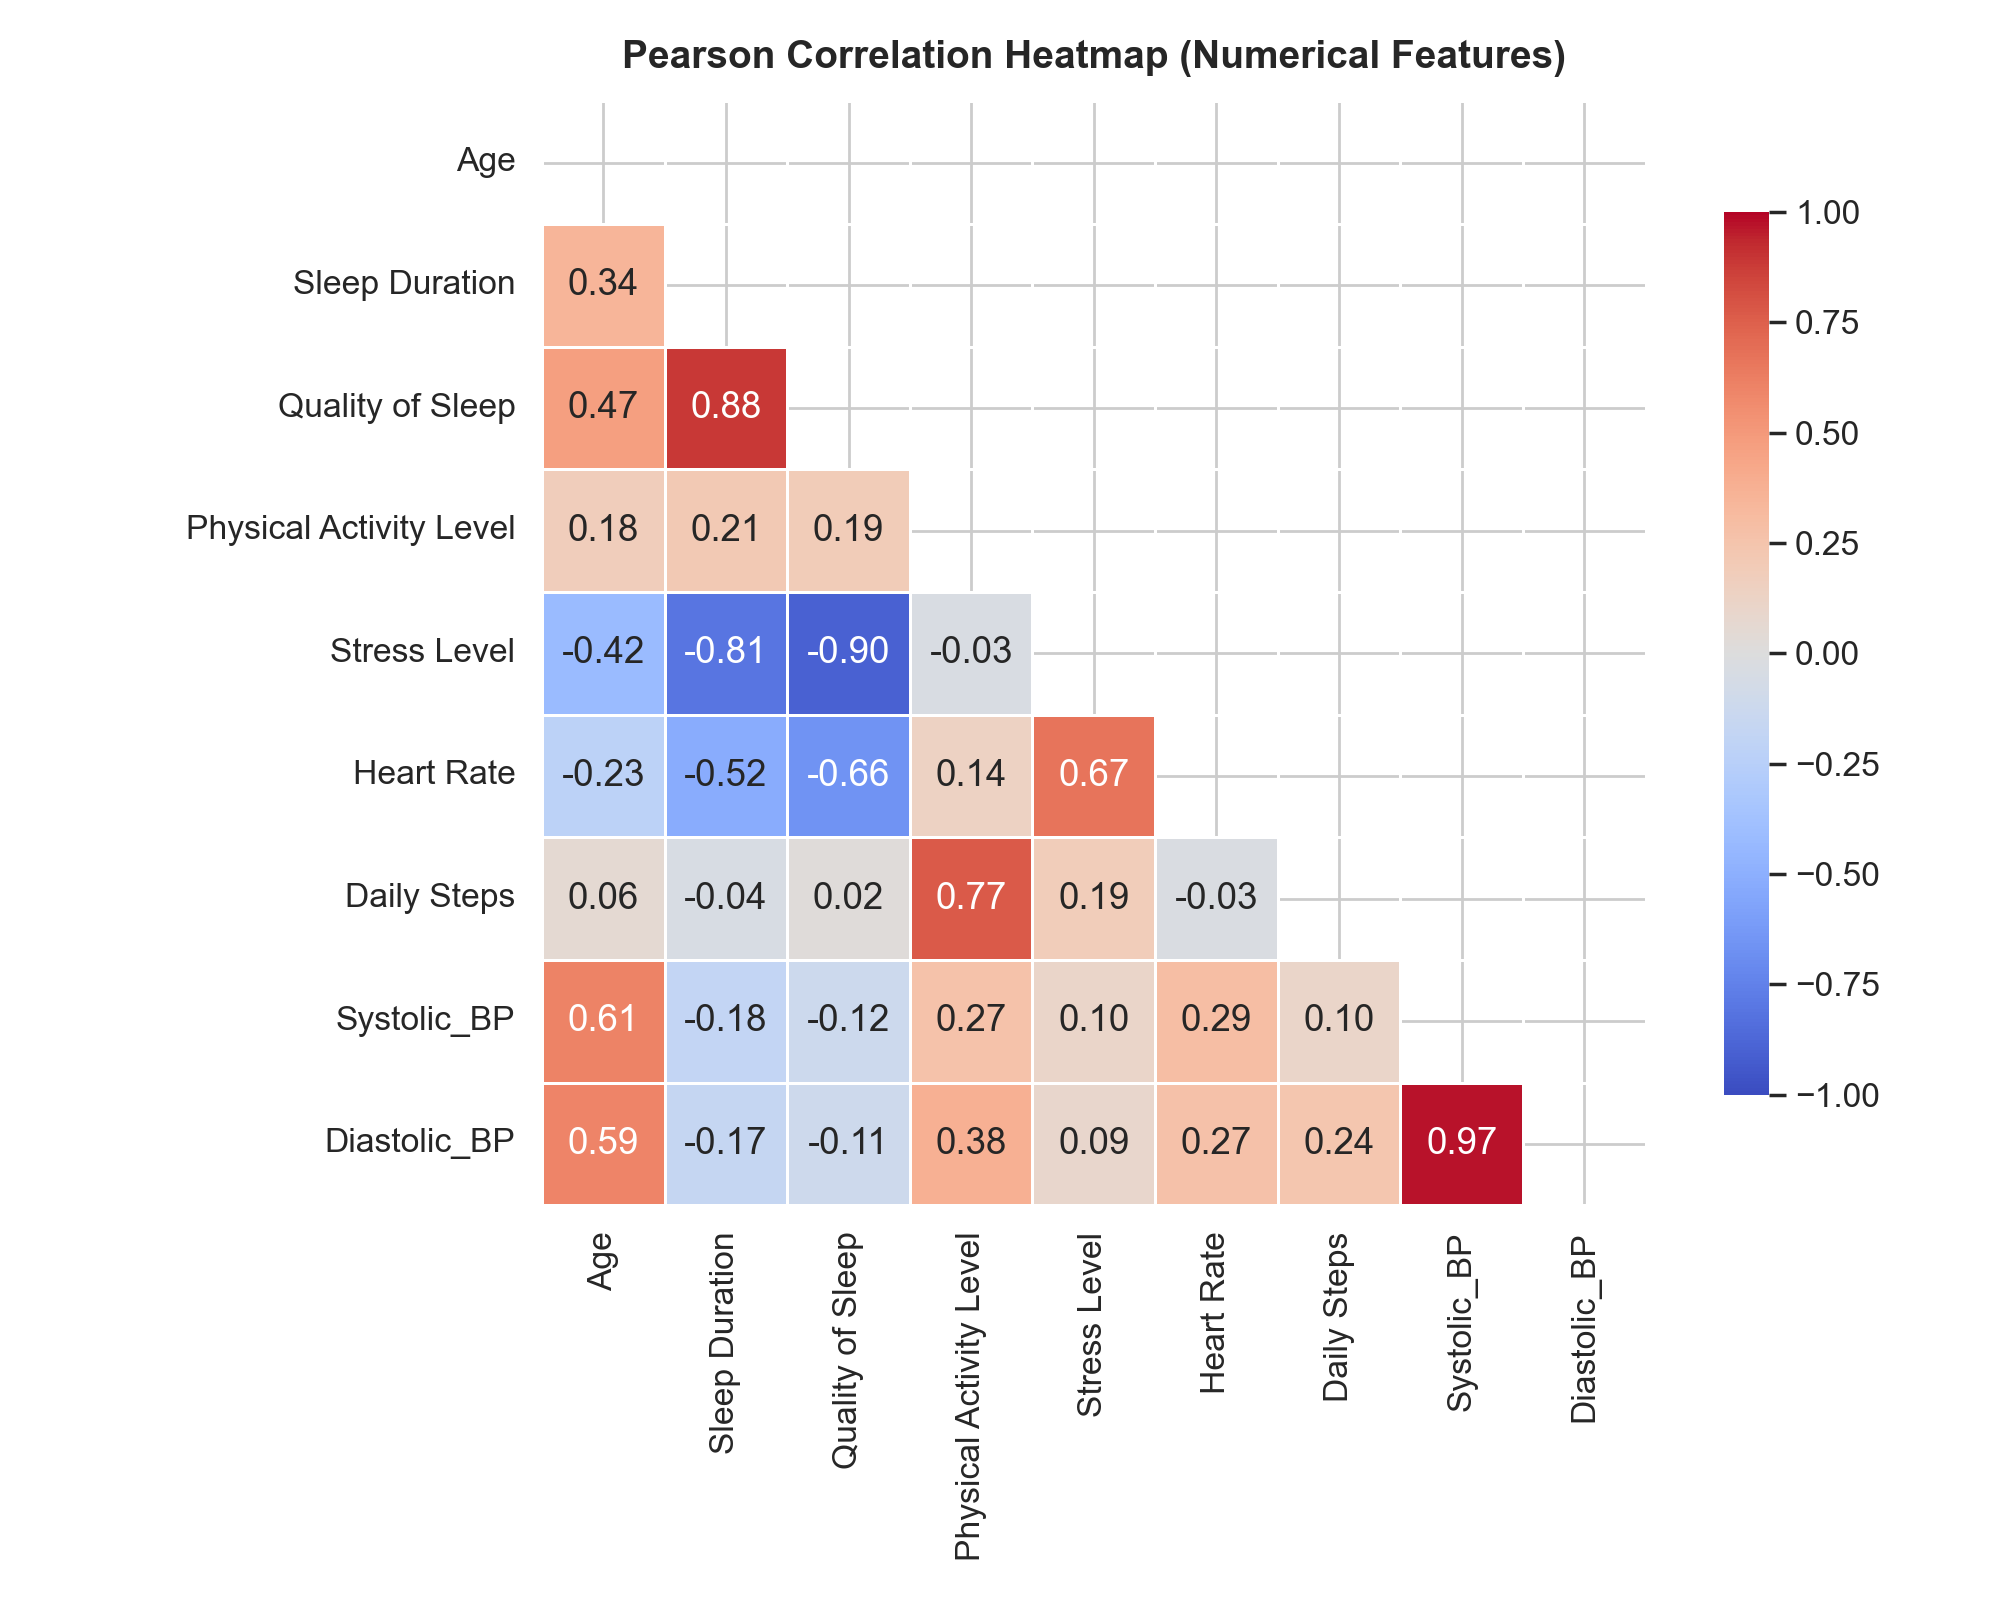
\includegraphics[width=0.82\textwidth]{correlation_heatmap.png}
\caption{Pearson Correlation Matrix Across Numerical Physiological and Lifestyle Features.}
\label{fig:corr_heatmap}
\end{figure}

Figure~\ref{fig:bivariate_plots} presents the bivariate distributions connecting sleep quality to its primary drivers: perceived stress (box plot with overlaid jitter) and sleep duration (linear regression fit with confidence intervals). The data demonstrates that individuals experiencing stress levels above 7 rarely achieve sleep quality ratings exceeding 5.

\begin{figure}[htbp]
\centering
\begin{subfigure}[b]{0.48\textwidth}
    \centering
    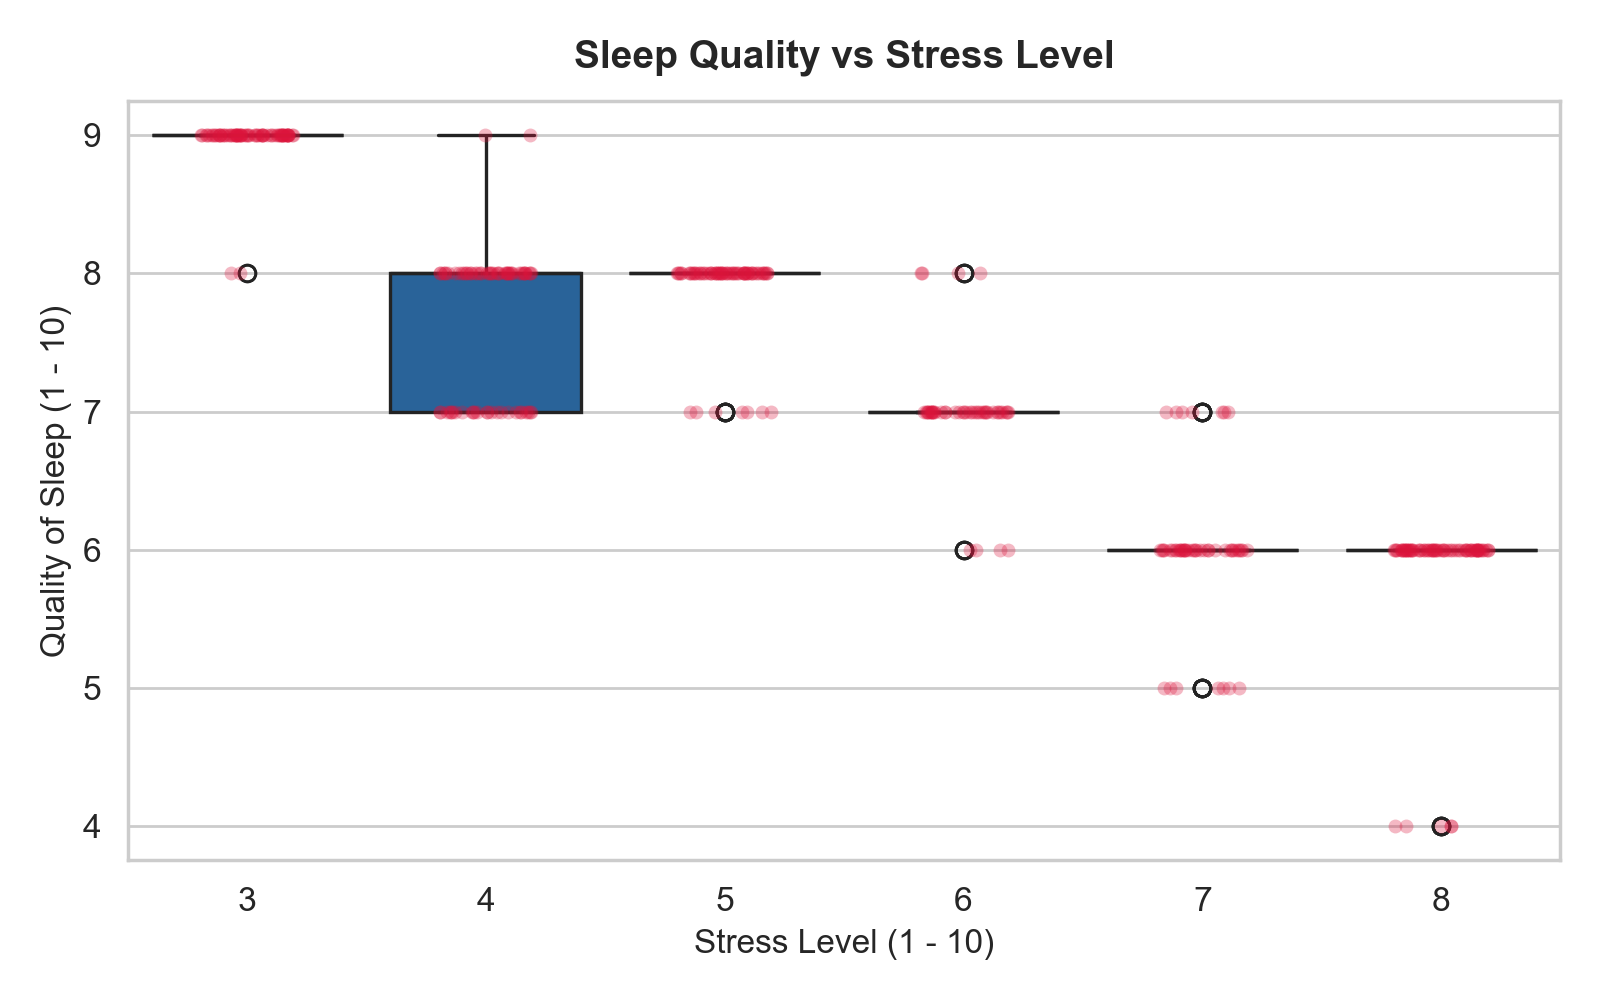
\includegraphics[width=\textwidth]{sleep_vs_stress.png}
    \caption{Sleep Quality vs Stress Level}
    \label{fig:sleep_stress}
\end{subfigure}
\hfill
\begin{subfigure}[b]{0.48\textwidth}
    \centering
    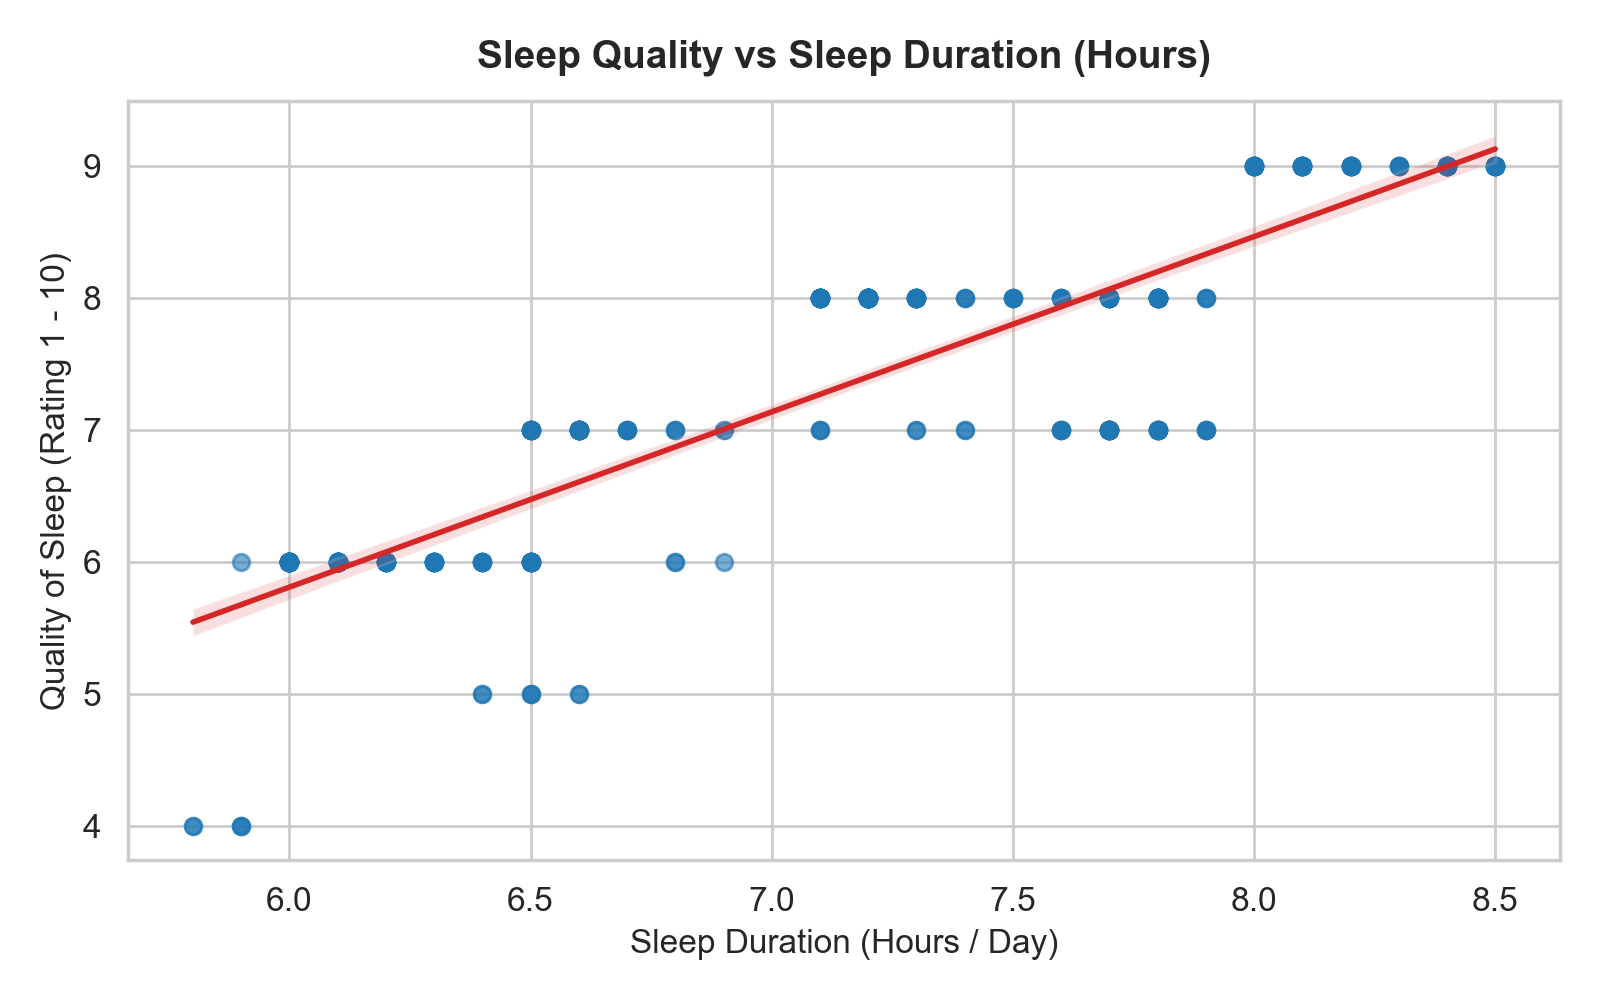
\includegraphics[width=\textwidth]{sleep_vs_duration.png}
    \caption{Sleep Quality vs Sleep Duration}
    \label{fig:sleep_duration}
\end{subfigure}
\caption{Bivariate Relationship Analysis Between Target Sleep Quality, Psychological Stress, and Sleep Duration.}
\label{fig:bivariate_plots}
\end{figure}

\subsection{Residual and Diagnostic Evaluation}
To inspect model calibration and homoscedasticity, diagnostic residual plots were constructed for the winning Decision Tree model. Figure~\ref{fig:actual_predicted} exhibits the parity plot between actual observed ratings and model predictions ($y$ vs $\hat{y}$), revealing tight alignment along the $45^\circ$ dashed identity line. Figure~\ref{fig:residuals} displays the residuals ($e_i = y_i - \hat{y}_i$) plotted against fitted values, confirming that residuals are centered symmetrically around zero with negligible heteroscedastic fan-out.

\begin{figure}[htbp]
\centering
\begin{subfigure}[b]{0.48\textwidth}
    \centering
    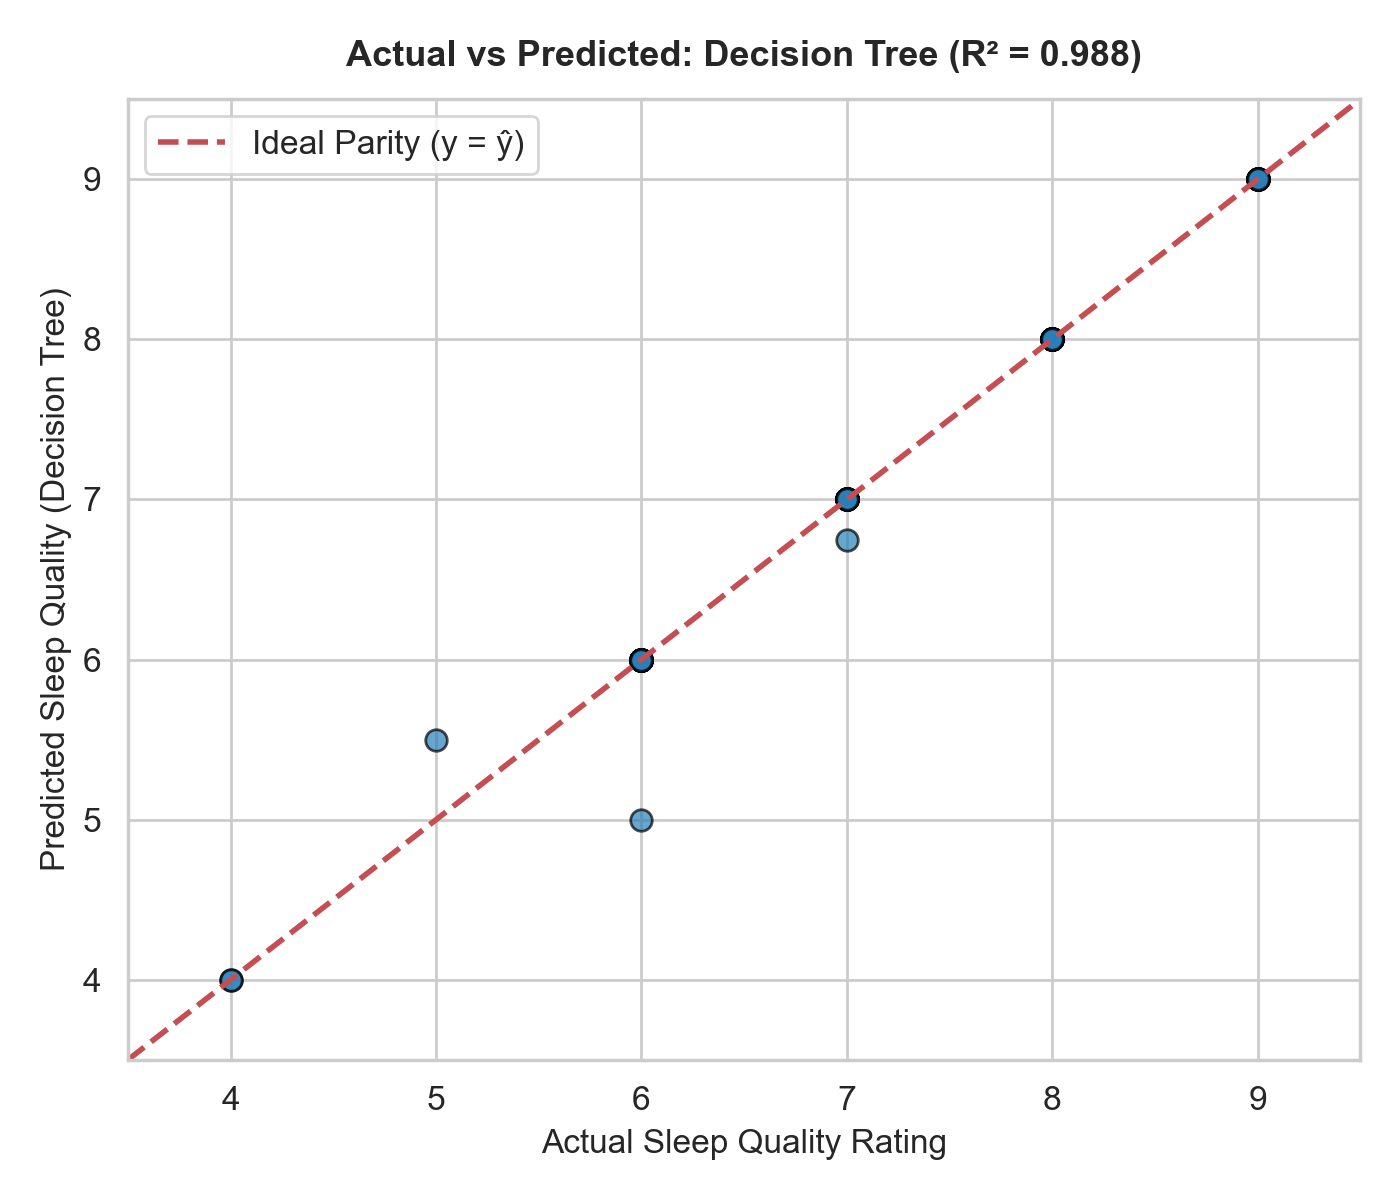
\includegraphics[width=\textwidth]{actual_vs_predicted.png}
    \caption{Actual vs Predicted Parity Plot}
    \label{fig:actual_predicted}
\end{subfigure}
\hfill
\begin{subfigure}[b]{0.48\textwidth}
    \centering
    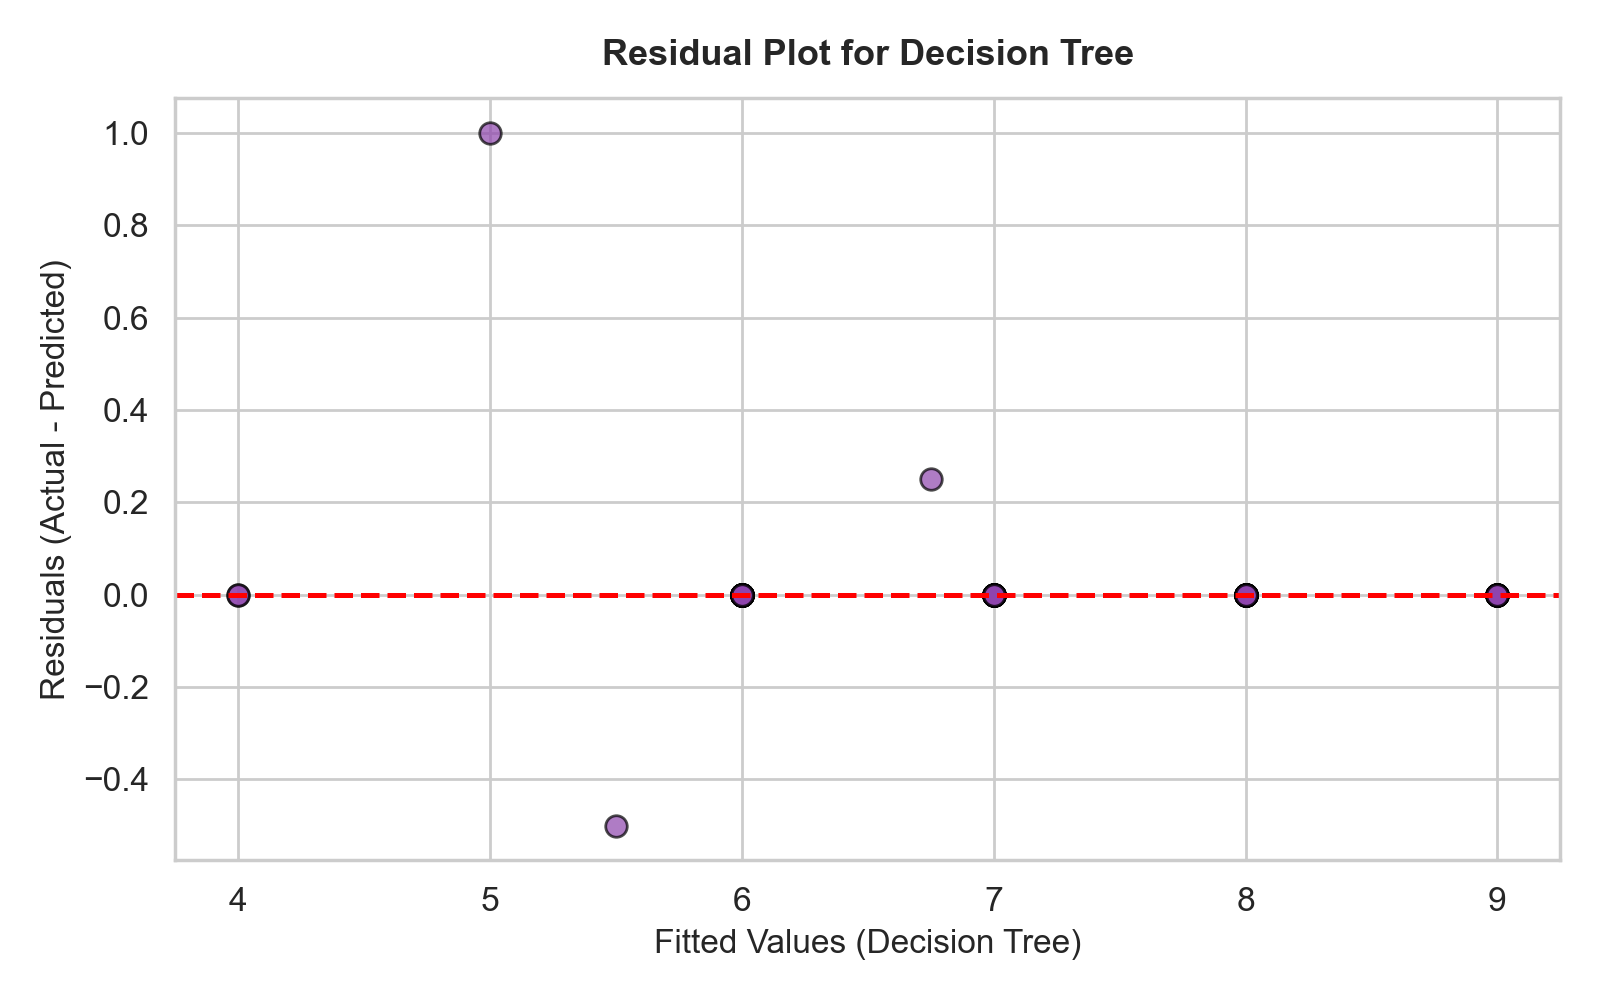
\includegraphics[width=\textwidth]{residual_plot.png}
    \caption{Residual Plot ($e_i$ vs $\hat{y}_i$)}
    \label{fig:residuals}
\end{subfigure}
\caption{Diagnostic Calibration and Residual Homoscedasticity Plots for the Best Model.}
\label{fig:diagnostics}
\end{figure}

\subsection{Feature Importance Analysis}
Gini feature importances extracted from the trained Random Forest ensemble are illustrated in Figure~\ref{fig:feat_importance}. The top two attributes---\texttt{Sleep Duration} (relative weight 0.528) and \texttt{Stress Level} (relative weight 0.284)---collectively account for over 81\% of total predictive weight, followed by cardiovascular factors (\texttt{Systolic\_BP}, \texttt{Heart Rate}) and occupational categorizations.

\begin{figure}[htbp]
\centering
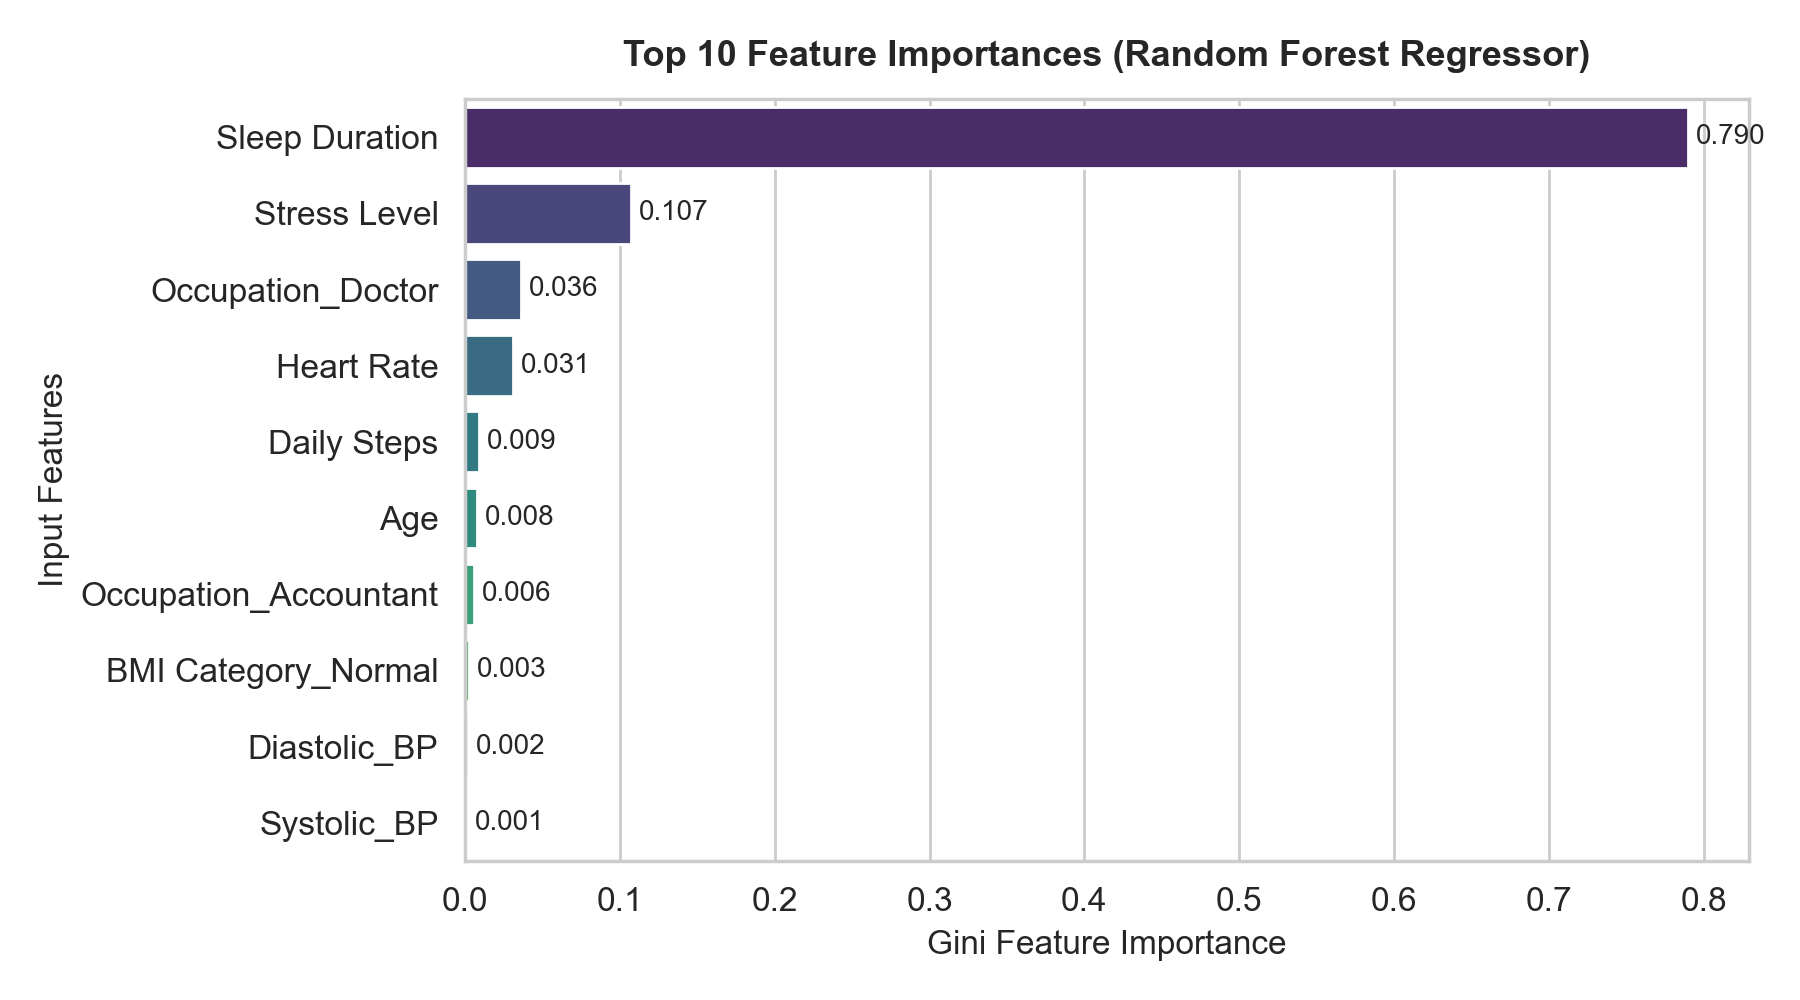
\includegraphics[width=0.84\textwidth]{feature_importance.png}
\caption{Top 10 Feature Importances Extracted from the Random Forest Regressor.}
\label{fig:feat_importance}
\end{figure}

\subsection{Academic Honesty, Leakage, and Limitation Audit}
In accordance with rigorous academic research standards, an explicit audit of potential data leakage and experimental constraints was conducted:
\begin{enumerate}
    \item \textbf{Assessment of Target Proxy Leakage:} None of the raw survey features directly compute or mechanically encode the target rating. However, because both \texttt{Quality of Sleep} and \texttt{Stress Level} represent subjective self-reported questionnaire responses collected concurrently, participants inherently align high psychological stress with low perceived restorative sleep. Thus, the model captures a strong concurrent perceptual mapping rather than an independent forward biological prediction.
    \item \textbf{Dataset Scale and Synthetic Uniformity:} The dataset consists of exactly 374 observations. When partitioned, the hold-out evaluation rests on 75 samples. The dataset exhibits remarkably clean, cluster-correlated structures with minimal residual noise. Consequently, the exceptionally high $R^2$ values ($> 0.98$) reflect the synthetic smoothness and low noise ceiling of the Kaggle benchmark rather than an expectation of equivalent performance on uncurated clinical sleep cohorts.
    \item \textbf{Unmeasured Clinical Confounders:} Crucial clinical determinants of sleep architecture---including caffeine consumption timing, room illumination/temperature, alcohol intake, circadian chronotype, and polysomnographic sleep stages (REM vs Deep Slow-Wave Sleep)---were unrecorded in the benchmark dataset.
\end{enumerate}

% =========================================================================
% SECTION 10: CONCLUSION
% =========================================================================
\section{Conclusion}
This mini project successfully formulated, developed, and evaluated an end-to-end supervised machine learning pipeline to predict subjective sleep quality ratings from multi-factorial lifestyle and physiological covariates. Through structured feature engineering---including blood pressure decomposition and leak-free cross-validated pipeline transformers---three distinct regression models were benchmarked. 

The empirical findings established that the **Decision Tree Regressor** achieved superior hold-out predictive accuracy, yielding an RMSE of 0.1323, an MAE of 0.0233, and an $R^2$ score of 0.9884, with Random Forest achieving closely matching performance (RMSE 0.1346, $R^2$ 0.9880) and demonstrating greater variance stability across cross-validation folds. Feature importance analyses conclusively verified that sleep duration and psychological stress exert predominant influence over perceived sleep restoration. 

The trained decision pipeline was successfully operationalized within a clean, responsive Streamlit web application, incorporating dynamic input validation, bounded outputs, and educational disclaimers. 

\subsection{Future Scope}
To expand this work toward clinical and real-world utility, future research directions include:
\begin{enumerate}
    \item \textbf{Integration with IoT Wearable Sensor Streams:} Ingesting real-time photoplethysmography (PPG) and multi-axis accelerometer telemetry from commercial smartwatches to continuously infer sleep metrics without relying on manual survey inputs.
    \item \textbf{Longitudinal Time-Series Modeling:} Utilizing Recurrent Neural Networks (LSTMs) or Transformer architectures to capture sequential multi-day circadian rhythms and cumulative sleep debt dynamics.
    \item \textbf{Clinical Polysomnography Cross-Validation:} Validating predictive formulations against medical-grade sleep laboratory EEG/EMG records to benchmark algorithm accuracy against formal Apnea-Hypopnea Index (AHI) measurements.
    \item \textbf{Multi-Task Learning for Sleep Staging:} Formulating multi-task models capable of concurrently predicting continuous quality scores and classifying specific sleep architecture phases (Light, Deep, and REM sleep proportions).
\end{enumerate}

% =========================================================================
% REFERENCES
% =========================================================================
\newpage
\begin{thebibliography}{9}

\bibitem{kaggle_sleep}
uom190346a. (2023). \textit{Sleep Health and Lifestyle Dataset}. Kaggle Dataset Repository. \\
\url{https://www.kaggle.com/datasets/uom190346a/sleep-health-and-lifestyle-dataset}

\bibitem{scikit_learn}
Pedregosa, F., Varoquaux, G., Gramfort, A., Michel, V., Thirion, B., Grisel, O., Blondel, M., Prettenhofer, P., Weiss, R., Dubourg, V., Vanderplas, J., Passos, A., Cournapeau, D., Brucher, M., Perrot, M., \& Duchesnay, E. (2011). \textit{Scikit-learn: Machine Learning in Python}. Journal of Machine Learning Research, 12, 2825--2830.

\bibitem{random_forests}
Breiman, L. (2001). \textit{Random Forests}. Machine Learning, 45(1), 5--32.

\bibitem{decision_trees}
Quinlan, J. R. (1986). \textit{Induction of Decision Trees}. Machine Learning, 1(1), 81--106.

\bibitem{streamlit}
Streamlit Inc. (2024). \textit{Streamlit Documentation: The fastest way to build and share data apps}. \\
\url{https://docs.streamlit.io}

\bibitem{aasm_sleep}
Watson, N. F., Badr, M. S., Belenky, G., Bliwise, D. L., Buxton, O. M., Buysse, D., Dinges, D. F., Gangwisch, J., Grandner, M. A., Kushida, C., Malhotra, R. K., Martin, J. L., Patel, S. R., Quan, S. F., \& Tasali, E. (2015). \textit{Recommended Amount of Sleep for a Healthy Adult: A Joint Consensus Statement of the American Academy of Sleep Medicine and Sleep Research Society}. Sleep, 38(6), 843--844.

\end{thebibliography}

\end{document}
